\documentclass[12pt, twoside]{report}

% Packages for equations and math symbols
\usepackage{amsmath}
\usepackage{amsfonts}
\usepackage{amssymb}

% Packages for figures
\usepackage{graphicx}
\usepackage{caption}
\usepackage{subcaption}
\usepackage{float}

% Packages for code
\usepackage{listings}
\usepackage{xcolor}

% Packages for links
% \usepackage{hyperref}
% \hypersetup{colorlinks=true,linkcolor=blue}

\definecolor{codegreen}{rgb}{0.1,0.6,0.1}
\definecolor{codegray}{rgb}{0.3,0.3,0.3}
\definecolor{codepurple}{rgb}{0.68,0,0.82}
\definecolor{backcolour}{rgb}{0.94,0.95,0.95}

% Python
\lstdefinestyle{python}{
    language=Python,
    backgroundcolor=\color{backcolour},
    commentstyle=\color{codegreen},
    keywordstyle=\color{magenta},
    numberstyle=\tiny\color{codegray},
    stringstyle=\color{codepurple},
    basicstyle=\linespread{1.0}\ttfamily\footnotesize,
    breakatwhitespace=false,
    breaklines=true,
    captionpos=b,
    keepspaces=true,
    numbers=left,
    numbersep=5pt,
    showspaces=false,
    showstringspaces=false,
    showtabs=false,
    tabsize=2,
}

\lstdefinestyle{inlinepython}{
    language=Python,
    basicstyle=\ttfamily\small,
    commentstyle=\color{codegreen},
    keywordstyle=\color{magenta},
    stringstyle=\color{codepurple},
    showstringspaces=false,
}

% Pseudocode
\lstdefinelanguage{Pseudocode}{
  morekeywords={for, to, end, if, then, else, while, do, repeat, until, return},
  morecomment=[l]{\#},
  morestring=[b]',
  sensitive=true
}
\lstdefinestyle{pseudocode}{
    language=Pseudocode,
    basicstyle=\ttfamily,
    keywordstyle=\bfseries,
    commentstyle=\itshape,
    xleftmargin=2em,
    aboveskip=1em,
    belowskip=1em,
}


% Double spacing
\usepackage{setspace}
\doublespacing

% Times New Roman font
\usepackage{times}

% Page margins
\usepackage[margin=1in]{geometry}

\begin{document}

% Title page
\title{CS 8770 \\ Neural Networks \\ Project 2}
\author{Drew Dahlquist \\ dgdtx5}
\date{April 25, 2023}
\maketitle

% Table of contents
\tableofcontents

% List of figures and tables (optional)
% \listoffigures
% \listoftables

% Chapter 1: Introduction
% \chapter{Introduction}

% Chapter 2: Technical Description
\chapter{Technical Description}

\section{Introduction}

For this project I decided to implement and explore LSTMs and find a dataset that naturally lends itself to 
sequence processing. I was able to find a decent quality dataset from the UCI Machine Learning repository on
bike sharing data that provides various features and the count of people who rented bikes for every hour over the 
span of 2 years, which gave me a good amount of data to work with, although more data would've been nicer.

I had a good amount of questions I wanted to attempt to answer during this project concerning LSTMs, as I'm
personally not very invested in predicting how many people will use bike sharing in a given hour.
I really wanted to build a good intution for designing and training LSTMs, particularly around how the
sequence length fed into the network influences training and inference, how the dimension of the cell/hidden states
influences the same as well as possibly gaining insight into what's going on in these mysterious features of LSTMs.
I looked into both some very natural ways for answering these questions 
(e.g., train, changing a hyperparameter, then train again) as well as some more exotic routes with the hopes
of finding them informative.

\section{Networks}

For my project I decided to study Long Short-Term Memory (LSTM) networks which are a type of 
recurrent neural network (RNN) architecture.
Unlike traditional RNNs, LSTMs can store information over longer periods of time, allowing them to better 
capture long-term dependencies in sequential data through the introduction of clever techniques allowing
gradients to better flow through the network without necissarily vanishing or exploding as is often the case
in traditional, vanilla RNNs.

At a high level, an LSTM module consists of several memory cells, which are responsible for storing information, 
and three gates - input, forget, and output gate - which control the flow of information into and out of the memory cells.
The input gate determines which parts of the input to let through to the memory cells.
It takes as input the current input, the previous hidden state, and a bias term, and produces an output between 0 and 1 
for each element of the input.
This output is then multiplied by the candidate values and added to the current memory cells.
Next the forget gate determines which parts of the previous memory cells to forget.
It takes as input the current input, the previous hidden state, and a bias term, and produces an output between 0 and 1 
for each element of the memory cells.
This output is then multiplied by the previous memory cells, and subtracted from the current memory cells.
Lastly, the output gate determines which parts of the memory cells to output as the hidden state.
It takes as input the current input, the previous hidden state, and a bias term, and produces an output between 0 and 1 
for each element of the memory cells.
This output is then multiplied by the current memory cells, and passed through a non-linear activation function to 
produce the hidden state.

The equations for the input gate, forget gate, and output gate in PyTorch are as given below:

\begin{align}
    i_t &= \sigma(W_{ii} x_t + b_{ii} + W_{hi} h_{t-1} + b_{hi}) \\
    f_t &= \sigma(W_{if} x_t + b_{if} + W_{hf} h_{t-1} + b_{hf}) \\
    o_t &= \sigma(W_{io} x_t + b_{io} + W_{ho} h_{t-1} + b_{ho})
\end{align}

Where $x_t$ is the current input, $h_{t-1}$ is the previous hidden state, and $W_{**}$ and $b_{**}$ 
are the weight matrices and bias terms.
LSTMs then compute the candidate values for the memory cells as follows:

\begin{align}
    g_t = \tanh(W_{ig} x_t + b_{ig} + W_{hg} h_{t-1} + b_{hg})
\end{align}

Finally, the new memory cells and hidden state are computed as follows:

\begin{align}
    c_t &= f_t \odot c_{t-1} + i_t \odot g_t \\
    h_t &= o_t \odot \tanh(c_t)
\end{align}

While necessary for properly defining/training an LSTM, these equations feel more at home in a diagram of LSTMs,
illustrating just how the flow of information is gated/connected within each module.
From the below figure we easily see how the cell state gets update by means of passing the
previous hidden state through the various gates, as well how the cell state influences the outgoing
hidden state. A key feature of LSTMs is the "gradient highway" afforded to the cell state which allows
gradients to backpropagate through many LSTM modules relatively untouched, making training much less painful
than with vanilla RNNs.

\begin{figure}[H]
    \centering
    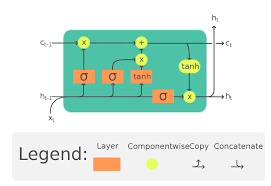
\includegraphics[width=0.75\textwidth]{figures/lstm fig.png}
    \caption*{LSTM (source: wikipedia.com)}
\end{figure}

\section{Data}

The dataset used is the Bike Sharing dataset coming from the UCI Machine Learning repository. The dataset consists of
two files containing various information such as date, season, year, weather, and most importantly, the
number of bikes rented by the hour or day (depending on which file you look at). For my project I chose
to use the hour.csv file only as this would allow me to pull more sequences for both training and testing.
I also did some manual feature selection via Microsoft Excel, and threw out some of the features I felt were
unnecessary such as instant, casual, registered, etc. In the end I was left with 11 features and 1 target variable –
the total count of riders during a given hour.

The main method of inference I focused on was given some sequence of previous hours, try to best predict the 
number of users that would rent bikes within the next hour. Although simple to state, this actually provided more
than enough material to work with in terms of exploring the internals of LSTMs, trying to answer some natural questions
I had going into this project, and also actually training a good network for perdiction.

In order to accomplish the above, I created my own custom PyTorch dataset class, which handles reading in the csv,
holding information about the sequence length being used, size of the data set, and retrieval of (feature, target) pairs - 
which in this case are sequences of the 11 features and the true count of users over the next hour.
For training/testing I stuck with a 4-to-1 ratio as I needed as much data for training as possible, and only
roughly cared about validation/testing for this project. As I discuss later in the project, while the LSTM
could properly learn, the data had a sufficient amount of noise so as to make highly accurate prediction very difficult.
However, the accuracy was still plenty close to notice the network was properly learning and to be an overall
acceptable machine.

\section{Training}

In an RNN, the same set of weights is used at each time step to process the current input and the previous hidden state.
As a result, the gradients that are computed during backpropagation must be propagated through time to all previous 
time steps in order to update the weights properly since the error at a given time step may depend on the 
inputs and hidden states from many previous time steps.

This is addressed via backprop through time (BPTT) by unrolling the RNN for a fixed number of time steps during training, 
creating a `deep' feedforward neural network with shared weights at each time step.
The gradients are then computed for each time step using the standard backpropagation algorithm, 
and the weights are updated using via optimization which is familiar from simpler MLPs or CNNs.

The unrolling process involves creating a copy of the RNN for each time step, and connecting the hidden state at 
one time step to the input at the next time step.
This creates a `chain' of RNNs that are connected through time and leads to the very cleverly named algorithm 
called `backpropagation through time'.
In theory this is perfect, however it causes some computational difficulties during training as it may lead to
the gradients becoming very small or very large as they are propagated through the many layers of the unrolled net,
making it difficult or impossible to update the weights properly.
This is known as the `vanishing gradient' and `exploding gradient' problems, respectively.

There are many ways to address this issue with gradients during training such as gradient clipping, different
activation functions, or by model respecification (i.e., LSTMs).
LSTMs address this key difficulty in training recurrent neural networks (RNNs) through the use of its gating mechanisms.
These mechanisms allow the network to selectively `remember' and `forget' information over time, 
which ideally prevents the gradients from becoming too small or too large during training.
Specifically, this is where LSTMs three gates - input, output, and forget gates - come in to play so as to 
control the flow of information through the network.
The input gate controls which information should be added to the cell state, while the forget gate decides 
which information should be discarded, and the output gate controls the output that is generated by the network.
Through the means of these gates, LSTMs can selectively update or ignore information at each time step,
which helps to prevent the gradients from vanishing or exploding as in vanilla RNNs.

% Chapter 3: Experiments and Results
\chapter{Experiments and Results}

\section{Sequence Length}

One of the first questions I had when starting to work with LSTM's was exactly what effect
the sequence length being fed into the network would have on the resulting inference. Intuitively,
it feels like our predictions should only get better as we feed in more prior data, since having a longer
sequence only adds information. However, I was still uncertain whether this would even be close to true,
since there are a lot of mechanics inside LSTMs that the presence of more sequential information may tamper
with.

In order to experiment with the effective of sequence length, I trained my LSTM until convergence with all
the same hyperparameters (hidden dim $= 5$, etc.) but only varied how many elements of the sequence I fed into it
for training and testing. Due to the hourly nature of my data, I opted to block of sequence length in natural intervals
such as 8 hours, 24 hours, etc. as it seemed the most natural considering its a time series. The results of this 
experiment is shown in the below plot.

\begin{figure}[H]
    \centering
    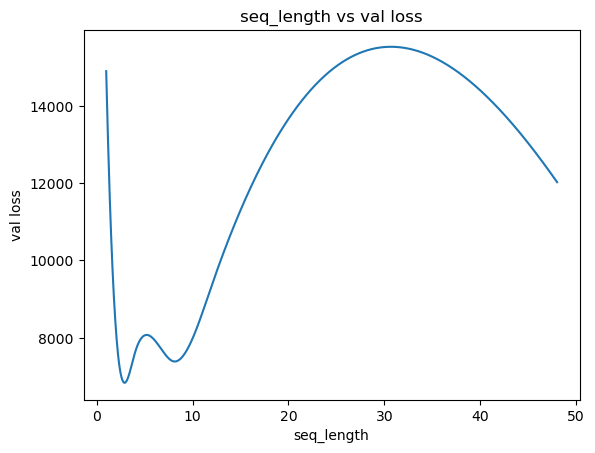
\includegraphics[width=0.75\textwidth]{figures/seq len vs val loss.png}
    \caption*{seq len vs val loss}
\end{figure}

It's easily seen my hypothesis of performance increasing with sequence length clearly didn't hold.
The initial decrease in val loss was entirely expected, as it's much easier to predict the next value
given the previous 2,4, or even 8, as opposed to just the previous 1.
What I wasn't planning on seeing was the sharp increase in val loss as the sequence length increases.
Furthermore, the decrease in validation loss after around 30 is most likely due to random variation from 
model initialization or train-validation splitting and not due to sequence lenght.

After some thought I feel the most likely explanation is that the longer sequence length affects the dynamics
of BPTT in a negative way resulting in more difficult training and thus worse performance on the validation set.
Ideally I would've liked to have multiple runs for each sequence length in order to marginalize any
effects from random initialization, randomization in batch presentation, and other conditions that generally
have little to nothing to do with the sequence length. However, training times on my laptop were much too long
to continue rerunning the same experiment to nail down a precise answer for optimal sequence length, so I took
the above conclusion of `it depends' as good enough and moved on.

\section{Hidden Dimension}

Expecting learning capacity to peak somewhere within $1 < h < 10$

\section{Visual(?) Dimension}

Below are visualizations of the high-dimensional cell state using t-SNE over the course of training the LSTM.
Each individual point is a prediction from the network on validation data and is colored according to the 
magnitude of the true label.

\begin{figure}[H]
    \centering
    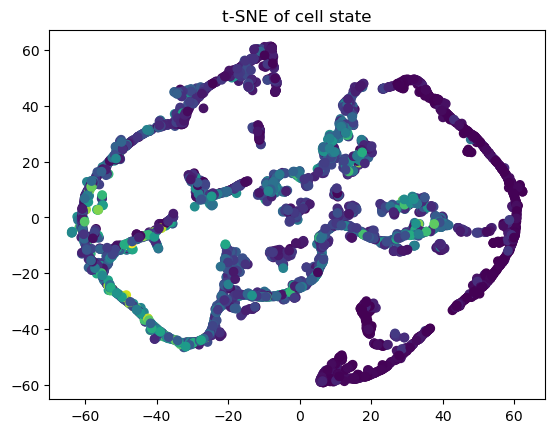
\includegraphics[width=0.65\textwidth]{figures/cell state evolution/1 epoch.png}
    \caption*{t-SNE of Cell State After 1 epoch}
\end{figure}

\begin{figure}[H]
    \centering
    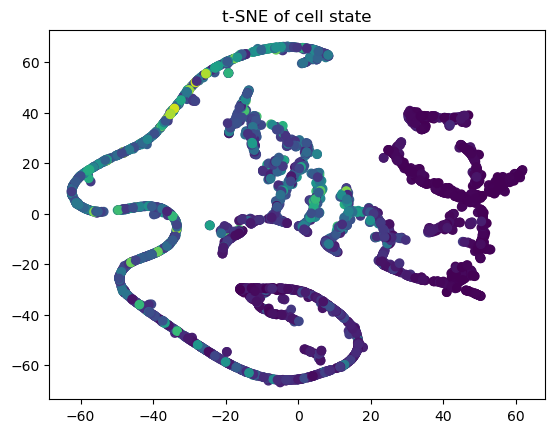
\includegraphics[width=0.65\textwidth]{figures/cell state evolution/5 epoch.png}
    \caption*{t-SNE of Cell State After 5 epochs}
\end{figure}

\begin{figure}[H]
    \centering
    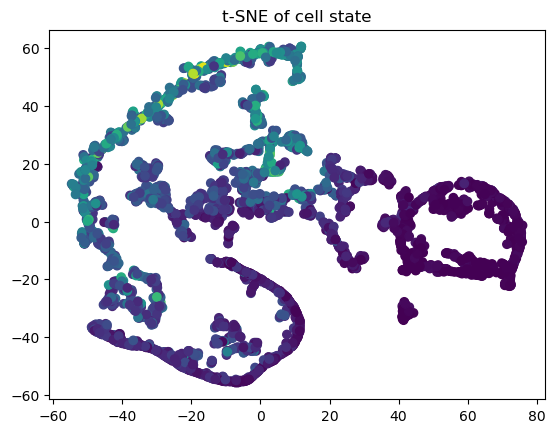
\includegraphics[width=0.65\textwidth]{figures/cell state evolution/15 epoch.png}
    \caption*{t-SNE of Cell State After 15 epochs}
\end{figure}


% Chapter 4: Reflection
\chapter{Reflection}


% References
\bibliographystyle{plain}
\bibliography{references}


\end{document}
